%{{{ Header
\documentclass[exam]{cs188}
\usepackage{verbatim}
\usepackage{fancyhdr}
\usepackage{mynotations}
\usepackage{booktabs}
\usepackage{setspace}
\usepackage{amsmath,mathrsfs}
\usepackage{multicol}
\usepackage{amssymb}
\usepackage{algpseudocode}
\usepackage{graphicx}
\usepackage{caption}
% \usepackage{subcaption}
\usepackage{array}
\usepackage{xcolor}
\usepackage{float}
\usepackage{enumitem}
\usepackage{mathcomp}
\usepackage{tabularx}
\usepackage{wasysym}
\usepackage{pbox}
\usepackage{pgfplots}
% \usepackage{algorithmic,algorithm}
\usepackage{tikz}
\usetikzlibrary{matrix,shapes}
\usepackage[normalem]{ulem}
\usepackage{multirow}
% \usepackage[inline]{enumitem}
%}}}

\title{Rattrapage}
\begin{document}
\newpage

% {{{ Questions de cours %
\begin{problem}[5]{(*) Questions de cours}
    \begin{enumerate}
        \item Soient $A$, $B$ et $C$ trois ensembles de $E$, développer les expressions suivantes:
        \begin{enumerate}
            \item $A\cap( B \cup C)$
            \item $A \cup( B \cap C)$ 
            \item $\left( A \cap B\right)^C$
        \end{enumerate}
    \item Soit $f:A\longrightarrow B$ une application de $A$ et $B$. Donner
        l'expression des ensembles suivants:
        \begin{itemize}
            \item $f(A)$.
            \item $f^{-1}(B)$.
        \end{itemize}

    \item Soient deux polynômes $P$ et et $Q$ dans $\Rr[X]$, donner la
        définition de:

        \begin{itemize}
            \item $\text{pgcd}(P, Q)$.
            \item $P$ est \textbf{irréductible}.
        \end{itemize}

\item Soit $E$ un $K$-espace vectoriel  et $F$ un sous ensemble de $E$. Donner
    une condition  suffisante pour que $F$ soit un \textbf{sous espace
    vectoriel}  de $E$.
    \end{enumerate}
\end{problem}
% }}} 
% Injections {{{ %
\begin{problem}[7]{Applications }
    \begin{enumerate}
        \item Soit $f:A\longrightarrow B$ une application. Pour toutes parties $A$ de
   $E$ et $B$ de $F$, montrer que:

   \begin{itemize}
       \item si $f$ est injective alors $f^{-1}(f(A)) = A$.
       \item si $f$ est surjective alors $f\left(f^{-1}(B)\right)= B$.
       \item Montrer que $f\left(f^{-1}(B)\right) = B \cap f(E)$.
   \end{itemize}
   \item Montrer que la fonction:
       \begin{equation*}
           \begin{array}{lll}
               \Rr\backslash\{-2\} & \longrightarrow &
               \Rr\backslash\{-2\}\\[4pt]
               x           &\longrightarrow & \dfrac{2x-1}{x+2}
          \end{array} 
       \end{equation*}
       \end{enumerate}

\end{problem}
% }}} Injections %
% Polynomes {{{ %
\begin{problem}[4]{Polynômes}
    On considère le polynôme:

    \begin{equation}
        P = X^4 -X^3 -5X^2 - X - 6
    \end{equation}
    
\begin{itemize}
    \item Vérifier que $3$ est une racine de $P$. 
    \item Si on vous donne le graphe de polynôme entre $[-6,6]$:

    \begin{figure}[htpb]
    \begin{center}
    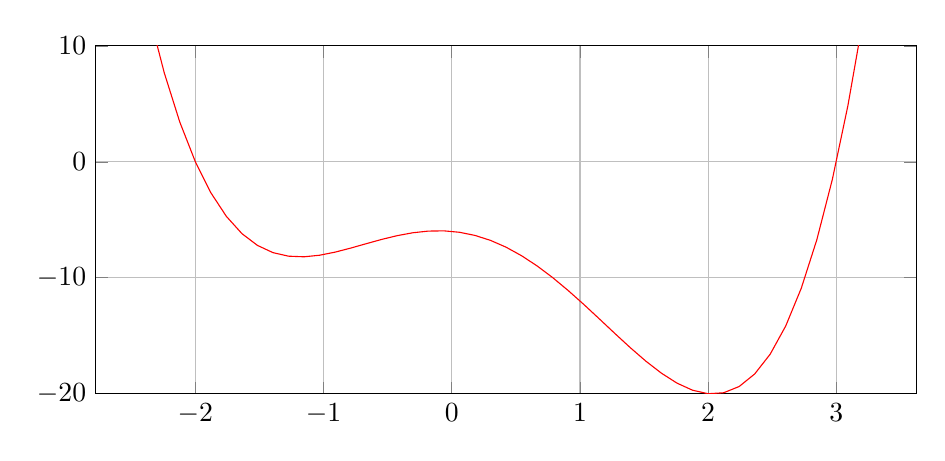
\begin{tikzpicture}[scale=1, transform shape]
        \begin{axis}[width=12cm, height=6cm, ymin=-20, ymax=10, grid]
         \addplot [
    domain=-6:6, 
    samples=100, 
    color=red,
]
{x^4 - x^3 -5*x^2 - x -6}; 
      \end{axis}  
    \end{tikzpicture}
    \end{center}
    \end{figure}
   Extraire une autre racine de  $\alpha$ de $P$. 

   \item En déduire une décomposition en facteurs \textbf{irréductibles}  de $P$
       dans $\Rr[X]$.
\end{itemize}
\end{problem}
% }}} Polynomes %
% Application linéaire {{{ %
\begin{problem}[4]{Applications linéaires}
    Soit $ f:\Rr^4\longrightarrow \Rr^4$ définie pour chaque $(x,y,z,t)\in
    \Rr^4$ par

    \begin{equation*}
        f(x,y,z,t) = \left(x-2y,\; x-2y,\;0,\; x-y-z-t\right)
    \end{equation*}

    \begin{enumerate}
        \item Montrer que $f$ est une application linéaire.
        \item Déterminer le noyau et l'image de $f$.
        \item A-t-on:

            \begin{equation*}
                \text{kern}(f) \oplus \text{im}(f) =\Rr^4
            \end{equation*}
    \end{enumerate}
\end{problem}
% }}} Application linéaire %
\end{document}
